\documentclass{article}

\usepackage[nonatbib]{nips_2017}
\usepackage{nips_2017}

% to compile a camera-ready version, add the [final] option, e.g.:
% \usepackage[final]{nips_2017}

\usepackage[utf8]{inputenc} % allow utf-8 input
\usepackage[T1]{fontenc}    % use 8-bit T1 fonts
\usepackage{hyperref}       % hyperlinks
\usepackage{url}            % simple URL typesetting
\usepackage{booktabs}       % professional-quality tables
\usepackage{amsfonts}       % blackboard math symbols
\usepackage{nicefrac}       % compact symbols for 1/2, etc.
\usepackage{microtype}      % microtypography
\usepackage{graphicx}

\usepackage[backend=biber]{biblatex}
\addbibresource{NIPS2017.bib}
\DeclareLanguageMapping{english}{american-apa}

\title{Combining curiosity and hierarchical reinforcement learning}

\author{
  Maria K.~Eckstein \\
  Department of Psychology \\
  UC Berkeley \\
  Berkeley, CA 94720 \\
  \texttt{maria.eckstein@berkeley.edu} \\  
  \And
  Tom Griffiths \\
  UC Berkeley \\
  Address \\
  \texttt{tom_griffiths@berkeley.edu} \\
  \And
  Anne GE Collins \\
  UC Berkeley \\
  Address \\
  \texttt{annecollins@berkeley.edu} \\
}

\begin{document}

\maketitle

\begin{abstract}
    Humans have the astonishing ability to acquire representations of their environment that allow them to learn from little and unorganized data often sparse in rewards, and to create multi-step goal-directed action plans efficiently. How this is possible is a puzzle both for research in psychology and artificial intelligence. We suggest that the combination of two specific mechanisms contributes to this ability: curiosity, the intrinsic motivation to explore novel states; and hierarchical structure, the ability to represent problems and actions across multiple levels of temporal abstraction. In order to test this hypothesis, we created a curiosity-driven hierarchical reinforcement learning agent (CHRL) and let it explore an unknown environment with hierarchical structure, and no rewards. The results are promising: The agent creates a hierarchical representation of actions across multiple time scales based on curiosity. Over learning, it performs action sequences of increasing duration and complexity, at fixed computational cost. This allows the agent to explore the environment more systematically than agents that lack curiosity, hierarchical structure, or both; to discover a larger number of meaningful states; and to visit these states more often. In future research, we plan to let human participants do the same task to identify the neural substrate underlying these mechanisms.
\end{abstract}


\section{Introduction}

Previous research in the cognitive sciences has suggested that two mechanisms are crucial for fast, efficient learning and for flexible, goal-oriented behavior: intrinsic motivation to explore specific aspects of the environment \cite{gopnik_scientific_2012, schmidhuber_formal_2010, lepper_undermining_1973}; and hierarchical structure of representations \cite{collins_reasoning_2012, anderson_act:_1996, miller_integrative_2001, frank_mechanisms_2012, chase_perception_1973, botvinick_model-based_2014}. Here, we argue that these two mechanisms go hand in hand, such that intrinsic motivation plays a role in learning hierarchical representations. One argument for this comes from neuroscience: Midbrain dopaminergic activity, known to be elicited by reward prediction errors \cite{schultz_neural_1997} and to act as a learning signal for the brain, is also elicited by novel events \cite{wittmann_striatal_2008}, suggesting that novelty too might trigger learning.

We hypothesize that the combination of intrinsic motivation and hierarchical learning can lead to an understanding of the environment that is more flexible than the mere prediction of reward in traditional reinforcement learning (RL) frameworks \cite{sutton_reinforcement_2017}. We hypothesize that agents can discover meaningful patterns of behavior without explicit reward signals, and learn to form multi-step plans without the need of a predictive model, as suggested by previous research in this domain \cite{machado_learning_2016, chentanez_intrinsically_2005, pathak_curiosity-driven_2017, kulkarni_hierarchical_2016, botvinick_model-based_2014}.%(Work on novelty: Deepak Pathak, Pulkit Arawal, Yael Niv, Schmidhuber; on hierarchy: Marlos Machado, Botvinick, Yael Niv, Pedro Tsividis; combination of both: Deep HRL paper)

We propose a curiosity-driven hierarchical reinforcement learning (CHRL) algorithm that explores a rewards-free environment based on its intrinsic curiosity, which is triggered by novel events. Once an event triggers the agent's curiosity (imagine an infant playing with a toy that suddenly makes a new sound), the agent creates an option \cite{sutton_between_1999} to try to reproduce the event (the sound). In order to achieve this goal, the agent learns, through trial and error, a specific option policy that leads to the event.% In this way, the agent will learn policies to control various aspects of its environment. %We model the process of option creation through hierarchical reinforcement learning, based on the options framework ().
The option policy operates over options one level of abstraction below, hierarchically all the way down to basic actions (producing a simple sound).
%In CHRL, only the most fundamental option policies are based on basic actions. More abstract option policies can be created by using option policies as the building blocks; this process can be repeated indefinitely, resulting in option policies of increasing abstraction, limited only by the temporal horizon of the agent. %In other words, the agent can learn to achieve abstract goals by breaking them down into sub-goals and sub-sub-goals, etc.
Crucially, CHRL relies solely on internally determined learning signals to guide its learning and behavior: 1) for learning option policies, the agent's internal pseudo-reward upon achieving its self-selected goal; and 2) the events' novelty for learning the value of options.

We show that...


\section{Methods}
 
\subsection{The MDP}

We created a learning environment with a hierarchical structure similar to more naturalistic tasks such as language or motor learning, which could realistically be presented to human learners in future experiments.
In the environment, the agent can execute a small number of "basic" actions that deterministically trigger unique "basic" (level-0) events in the environment. In addition, certain sequences of basic actions trigger a "level-1" event, in addition to the basic event. Similarly, certain sequences of level-1 events produce level-2 events, etc. %This is similar to the structure of language learning: there, the agent progresses from learning phonemes (basic actions) to combining phonemes into syllables (learnign to produce level-1 events), syllables into words (level-2 events), words into phrases, phrases into sentences, etc.

Formally, we define the set of the agent's $k_0$ basic actions $\mathcal{A}_0 = \{a_{0, 1}, a_{0, 2}, \ldots, a_{0, k_0}\}$. We define each element of the state space $\mathcal{S}$ as the tuple $(f_{0, 1}, \ldots, f_{0, k_0}, \ldots, f_{L, 1}, \ldots, f_{L, k_L})$, defined by binary features $f_{l, i}$ for levels $l$ and index $i$. When the agent selects $a_{0,i}$ at trial $t$, the new state's level-0 features are $f_{0,i}=1$ and $\forall j \neq i, f_{0,j}=0$: action $a_{0, i}$ changes the feature $f_{0, i}$ from 0 to 1 - this change in feature is "event" $e_{0, i}$. Furthermore, at any level $l$, there is at most one index $i$ such that $f_{l,i}=1$: all features $f_{l, j}, \forall j\neq i$ are set to $0$ before feature $f_{l, i}$ is set to $1$. Last, at each level $l$, there exist triplets $i \neq j$ and $k$ such that if $f_{l,i}(t)=1$ and $a(t)=a_{l,j}$, then $f_{l+1, k}=1$: lower-level actions in specific states can trigger higher-level events, in addition to their own level's event.

\subsection{Event novelty and curiosity}

We assume that the agent explores the environment based on its intrinsic curiosity. Curiosity is determined by event novelty and determines the agent's propensity to select an event as a target of exploration. Formally, novelty of event $e$ is defined as $n_e = e^{-\lambda i_e}$ where $i_e$ is the number times event $e$ has occurred since the agent's first encounter with the environment and $\lambda$ is the agent's rate of novelty decay. We assume that curiosity $c_e$ about an event is learned through reinforcement, with delay-discounted novelty serving as teaching signal: $c_e(t+1) = c_e(t) + \alpha (\gamma^{j_e} n_e(t) - c_e(t))$ whenever event $e$ occurs. Here, $\alpha$ is the agent's learning rate; $\gamma$ is the agent's discounting of the future, and $j_e$ is the number of time steps spent within option $o_e$, which led to event $e$ ($j_e = 0$ when event $e$ happened without executing option $o_e$; $j_e = 1$ when $e$ is a basic event). In order to select specific events as sub-goals, the agent uses $\epsilon$-greedy selection based on its curiosity.

\subsection{Option creation}

Initially, the agent possesses only "basic actions". When a higher-level event occurs for the first time, it is added to the agent's option space as a potential sub-goal. The option policy of the new sub-goal can use all options at the level below to reach the new sub-goal. Formally, the agent's initial option space $\mathcal{O}$ comprises only basic actions, $\mathcal{O} = \mathcal{A}_0$. When event $e_{l, i}$ occurs for the first time, the agent's option space is extended by the option $o_{e_{l, i}}$ targeted at producing event $e_{l, i}$: $\mathcal{O} = \mathcal{O} \cup o_{e_{l, i}}$. Option $o_e$'s initiation set $\mathcal{I}$ is the whole state space, $\mathcal{I} = \mathcal{S}$. The termination condition is the following. An option terminates with probability $p=1$ for all states in which $f_e = 1$ (in which the target event $e$ occurred) and $p = \epsilon_T$ in all other states. The action space of $l$th level option $o_{e_{l, i}}$ comprises all options $o_{e_{l-1, .}}$ at level $l-1$. For example, the policy of a level-1 option $o_1$ operates on the action space comprising all basic actions $a_{0, i} \in \mathcal{A}_0$. 

\subsection{Learning option policies}

When the agent selects a specific event $e$ as sub-goal, the option policy $o_e$ controls action selection until the option terminates. The option policy learns through temporal-difference learning \cite{sutton_reinforcement_2017} which actions lead to the sub-goal. After option termination, the agent's curiosity about the sub-goal is updated based on the novelty of the produced event (or the failure to produce the event).

%Formally, option $o$'s policy $\pi_o$ is $\epsilon$-greedy over within-option values $V_o$. $V_o$ are defined by the weights $\theta$ of the binary features $f(t)$ that describe the state of the environment at time $t$, $V_o^{t}(s_t, a_t) = \theta^T f^t$. 
%$V_o$ are updated through temporal difference learning on the weights $\theta$: $\theta^{t+1} = \theta^t + \alpha (r_p + \gamma \max_a(V_o^{t}(s^{t+1}, a)) - V_o^{t}(s^t, a^t))$; here, the pseudo-reward $r_p = 1$ when $e$ occurred (and the option terminates) and $r_p = 0$ otherwise; $V_o(s^{t+1},\cdot) = 0$ when the option terminates. 

\subsection{Simulations and competing algorithms} \label{Comparison agents}

We simulated the agents' behavior over environments designed to be sufficiently complex to challenge learning: $5$ hierarchical levels and $5$ possible events at each level. All higher-level events were triggered by sequences of two subsequent events at the level directly below.%; rules were allowed to overlap, but could not be identical, e.g., when one rule was $e_{l_2} + e_{l_3} \rightarrow e_{l+1, 1}$ ($e_{l_2}$ followed by $e_{l_3}$ produces $e_{l+1, 1}$), another rule might be $e_{l_2} + e_{l_4} \rightarrow e_{l+1, 2}$). 

Agents explored the environment for 400 time steps, i.e., executing 400 basic actions. We used the following parameter settings for all agents: $\alpha = 0.3$, $\lambda = 0.3$, $\gamma = 0.9$, $\epsilon = 0.2$, and $\epsilon_T = 0.1$. We obtain similar results with different parameter sets. The data shown below are based on the average performance of 99 agents in a single environment (section \ref{Results CHRL}), and the average performance of 3 agents in 15 environments (section \ref{Results compare all}). The results hold for individual agents and environments.

To investigate the importance of both hierarchical structure and novelty seeking to behavior, we compared CHRL to three other agents without one or both of these mechanisms. Reward-based agents used a reward function defined as the number of current events instead of novelty for learning; flat agents did not create options.%The reward-based hierarchical agent created and employed options in the same way as the CHRL agent, but used reward $r$ instead of novelty as an update signal for option values; we define reward as the number of events produced in a given trial.
%The novelty-based flat agent selected options based on curiosity like the CHRL agent, but it did not create or use options. Therefore, $O = A_0$ and $S = S_0$. The reward-based flat agent is a combination of these two agents, with neither options nor novelty-based learning.


\section{Results}

\subsection{Behavior of the CHRL agent} \label{Results CHRL}

Through exploration and experience of novel events, the CHRL agent acquired several different, hierarchically structured option policies. Thereby, option policies targeted at simpler events were learned faster than for complex events, and final policies were also more accurate (data not shown).

In addition, as expected, the agent's curiosity decreased fastest for basic events (level 0), and increasingly slowly for higher levels of abstraction (fig. \ref{CuriosityFigure}). In other words, the simpler an option, the faster the agent lost interest in executing it for it's own sake. Importantly, this does not imply that the agent executed simple options less often overall: on the contrary, the rate of all abstract events increased over time (fig. \ref{CEvents}). This is because simple options form the building blocks of all abstract options that become more interesting.

%Finally, the agent showed some kind of "specialization": The higher the level of abstraction, the fewer events it discovered. The reason for this is that once a higher-level option is discovers, it dominates behavior and less exploration
%level-1 events required the sequential execution of two specific level-0 actions, whereas level-4 events required the sequential occurrence of 2 level-3 events, which correspond to 4 level-2 events, and eventually 16 basic actions. 

\begin{figure}[h]
	\centering
	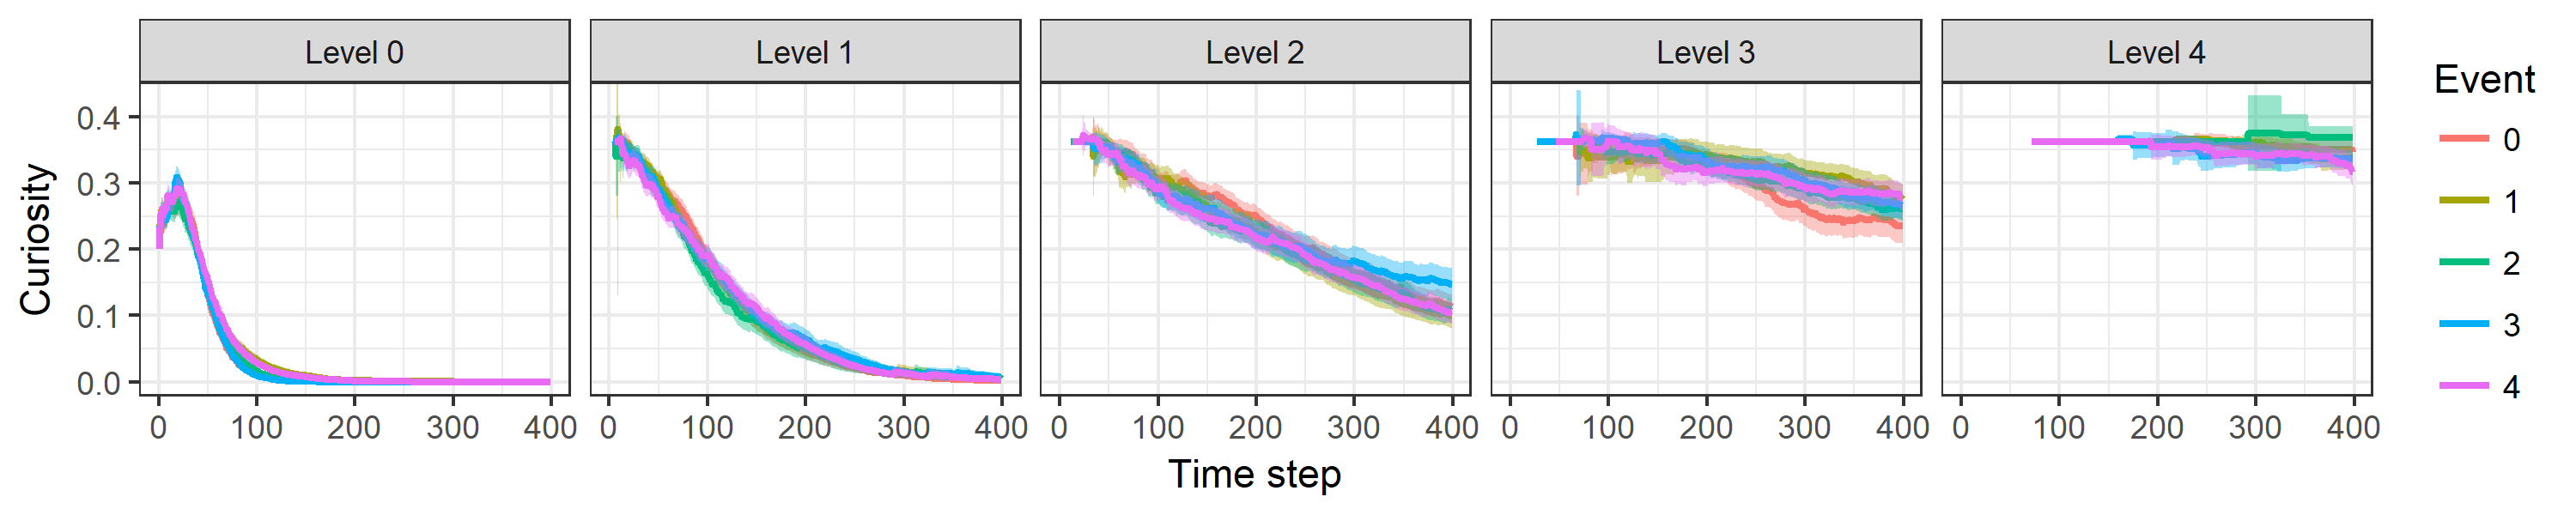
\includegraphics[width=\linewidth]{ACuriosity.png}
	\caption{Curiosity for events decreases over time. Shaded areas indicate the standard error of the mean. The higher-level an event, the slower curiosity decreases. The environment contained 5 different events at each level of abstraction. The agent does not usually discover all events (e.g., only one event was discovered at level 4.)}
	\label{CuriosityFigure}
\end{figure}

\subsection{Comparison of the CHRL agent and other agents} \label{Results compare all}

We compared CHRL's behavior to three other three agents (see section \ref{Comparison agents}). CHRL discovered a larger number of different events than the other agents, and at a faster rate (fig. \ref{CEvents} A). Both the novelty-based flat agent and the reward-based hierarchical agent outperformed the reward-based flat agent, suggesting that both curiosity and hierarchical structure were crucial for effective exploration.

The reason for the exploration advantage is CHRL's specific pattern of curiosity, with larger curiosity for higher-level events. Due to that, the agent will execute more higher-level options (fig. \ref{CEvents} B), which increases the probability of observing events at higher levels. 

\begin{figure}[h]
	\centering
	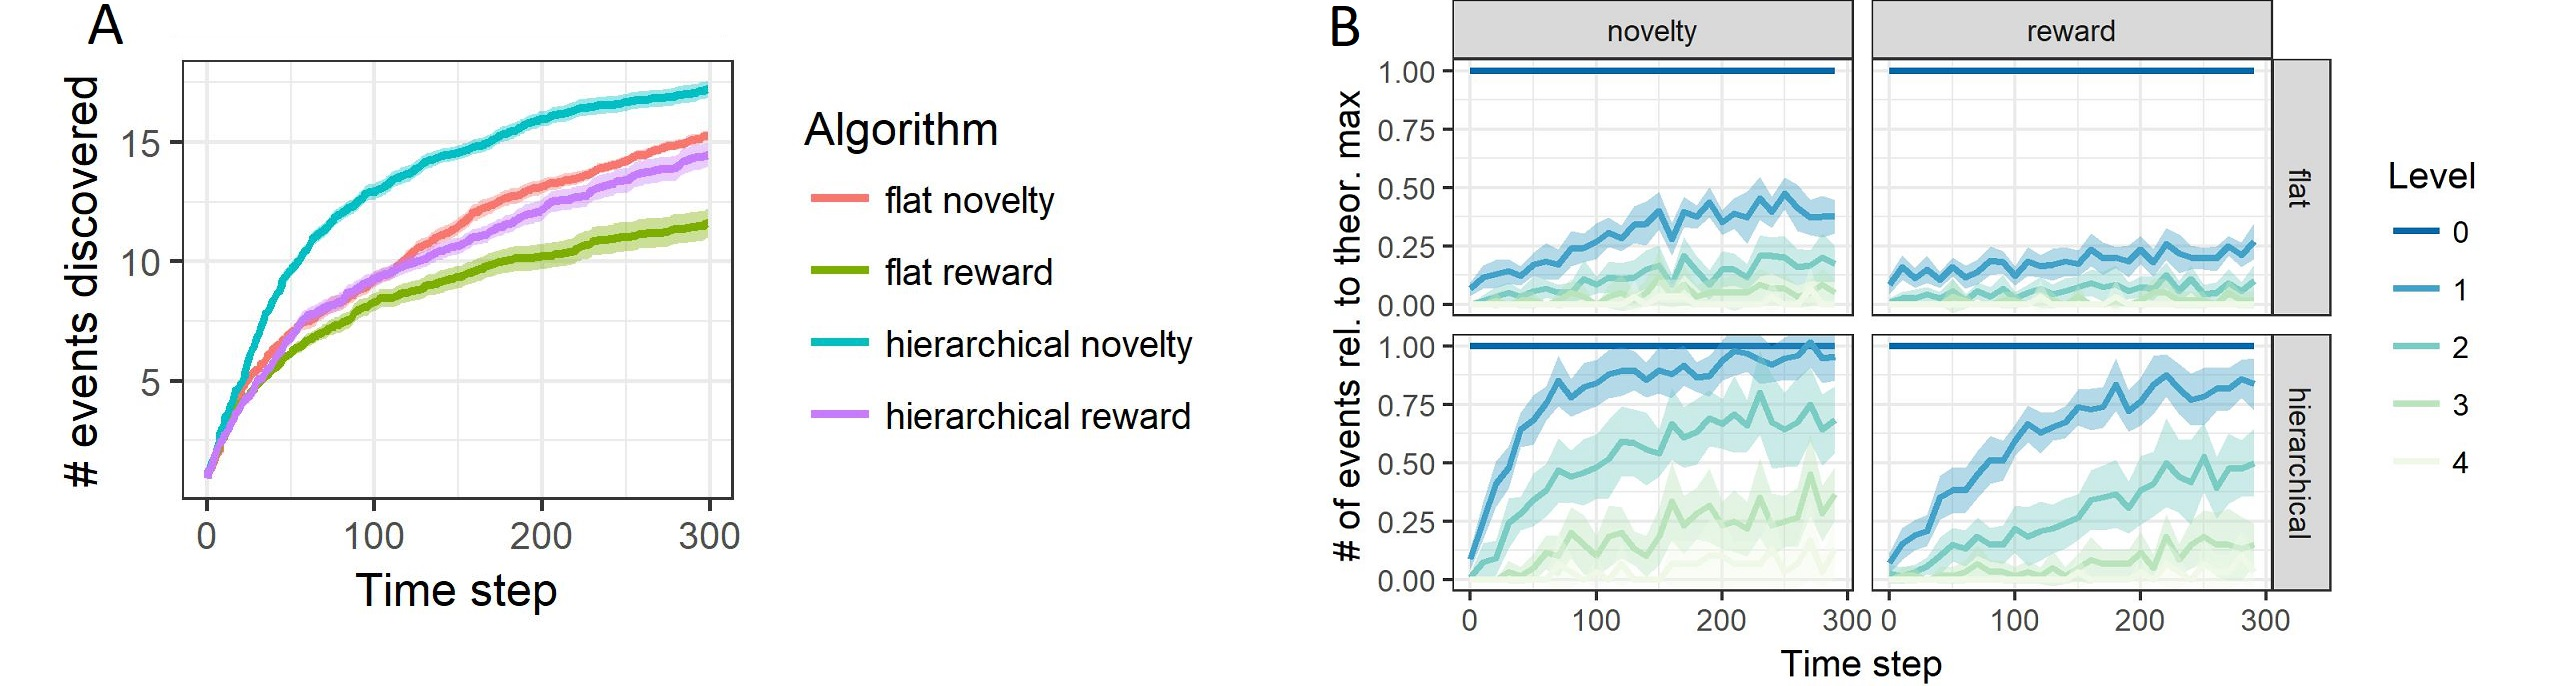
\includegraphics[width=\linewidth]{CEvents.jpg}
	\caption{A) Number of events discovered by each of the four agents over the course of 300 time steps. B) Number of events that occurred in each bin of 10 time steps, relative to theoretical maximum (theor. max. for level-0: 10 / 10; level-1: 5 / 10; level-2: 2.5 / 10; etc.). Shaded areas indicate 95\%-confidence interval of the mean.}
	\label{CEvents}
\end{figure}


\section{Conclusion}

We have stated that two factors crucially contribute to human ability to form goal-directed, abstract action plans in environments that are unorganized and sparse in rewards: curiosity-driven exploration and the creation of hierarchical option policies. Both factors have been the target of various research in the cognitive sciences and, more recently, have gained interest in computer science and artificial intelligence research.

In order to test this hypothesis, we implemented CHRL, a reinforcement-learning algorithm that is driven by curiosity and that has the ability to create hierarchical option policies. This agent indeed shows characteristics expected from human learners. For example, the agent's curiosity declines fastest for basic events, but slower for more abstract events. This is because option policies become better and better at producing their goal events, such that the corresponding events occur more frequently and, over time, decrease in novelty. This leads to a decrease in the agent's intrinsic motivation to explore events further once they are understood. Nevertheless, this process does not slow down learning: Acquiring new skills, rather than reducing motivation and slowing down exploration, opens up new possibilities of learning even more abstract skills. Similarly, in the human domain, whereas an infant might be curious about individual sounds, a toddler might be interested in children's songs, and an adult in twelve-tone music or Italian Opera. 

We then moved on to compare the CHRL agent to flat and reward-driven agents. The CHRL agent outperformed the other agents in terms of exploration efficiency, discovering a larger number of different events in the given environment. It also produced an overall larger number of abstract events than the other agents. This is especially remarkable because two of the other agents were rewarded depending on the number of abstract events, whereas CHRL was not. This highlights how powerful novelty can be as a learning signal.

One limitation of the current work is that we did not compare our agent to other implementations of option learning (cite who? -> RLDM). The reason for this is that our main interest lies in understanding human intelligence, rather than creating artificial intelligence. Nevertheless, it would be interesting to compare our framework to others. It would be especially exciting to integrate advances from this field, such as curiosity based on prediction rather than counting. 

We have also assumed very simple mechanisms for detecting events and measuring novelty. Although this limits the usefulness of the algorithm in AI problems, it is an advantage for our purposes because it gives us great experimental control. Once translated into a human task, this will allow us to explore how various factors contribute to hierarchical learning, for example the number of basic actions, the length of options, and the depth of necessary abstraction (number of levels). 

Our goal for future work is to tweak the algorithm until it shows human-like behavior in this task, reproducing the overall pattern as well as typical mistakes. We can then extract trial-by-trial measures from the algorithm, for example curiosity-prediction errors, and regress them again physiological measures, such as functional magnetic resonance imaging (fMRI) data obtained from participants doing the task. This might allow us to study the neural underpinnings of the observed human behavior, localizing specific functions within the brain.

Taken together, by creating the hierarchical novelty-seeking agent, we hope to show that learning of meaningful behavior can be driven by learning itself, rather than external rewards. In this framework, the learner produces the crucial learning signals itself, by selecting actions that over time reduce novelty. In other words, this learner balances the search for novelty with reducing prediction errors. It explores the environment in a systematic way, forms "hypotheses" and conducts "experiments", in order to learn more, just like is expected from a human learner.

\printbibliography

\end{document}